\lhead{\emph{Conceptos teóricos}}
\chapter{Conceptos teóricos}

Es necesario conocer una serie de conceptos clave antes de pasar a los diferentes aspectos de análisis y desarrollo del sistema. Se incluye además en cada apartado una sección que indica la aplicación final de cada uno de los conceptos teóricos en el sistema final.

\section{Computación distribuida}

Un sistema distribuido es aquel conformado por un conjunto de nodos independientes que son percibidos como una entidad única y coherente por el usuario final. Dicha definición implica dos conceptos de importancia:

\begin{itemize}
  \item \textbf{Autonomía}: los diferentes integrantes cuentan con un alto grado de autonomía entre sí, y por tanto se deben diseñar e implementar mecanismos de comunicación entre los mismos que formarán parte del núcleo del sistema, y cuyo diseño tendrá consecuencias directas en el funcionamiento final del mismo.
  \item \textbf{Transparencia}: Las diferencias entre diferentes nodos deben ser invisibles para los usuarios finales, así como la gestión de fallos y la posterior recuperación, así como la uniformidad a la hora de interactuar con el sistema. Según \citationneeded las siguientes propiedades deben contar con un grado de transparencia alto:\footnote{En numerosas ocasiones las propiedades de un sistema hacen desfavorable el cumplimiento de todos los requisitos de transparencia. Un ejemplo sería la transparencia de traslado en el sistema DNS.}:
\label{transparencia}
  \subitem \textbf{Acceso}: La forma de almacenamiento y gestión de los recursos e información presentes en el sistema debe ser completamente transparente.
  \subitem \textbf{Localización}: La localización física del sistema no debe ser de relevancia para el uso del mismo.
  \subitem \textbf{Migración}: El cambio de plataforma debe ser transparente para el usuario (ejemplo: cambio del sistema operativo).
  \subitem \textbf{Traslado}: El hecho de que un sistema se esté trasladando de un lugar a otro no debe afectar al usuario final.
  \subitem \textbf{Replicación}: El numero de elementos redundantes en un sistema es desconocido para el usuario final.
  \subitem \textbf{Concurrencia}: Un usuario no debe percibir la presencia de otros agentes interactuando con el sistema.
  \subitem \textbf{Gestión de errores}: En caso de fallo, el usuario final no debe percibir el mismo, ni el proceso de recuperación consecuente (ver \ref{teoria:autoadministracion}.
\end{itemize}

Generalmente los sistemas distribuidos son fácilmente escalables gracias a la autonomía de cada nodo, y los mecanismos de transparencia permiten crear sistemas heterogéneos de forma sencilla, en ocasiones apoyados en capas \textit{middleware} (ver \ref{teoria:middleware}) que posibilitan dicha transparencia.

Otro concepto importante en el desarrollo de sistemas distribuidos es la ``franqueza'' (\textit{openness}) de los mismos. Un sistema ofrece una serie de servicios gracias al uso de un conjunto de reglas conocidas por todos los participantes, generalmente recogidas en estándares de acceso público que definen la sintaxis y semántica de los servicios, conocidos como lenguajes de especificación de interfaz (\textit{Interface Definition Language}), tales como CORBA\cite{corba} o el \textit{IDL specification language}\cite{idl} (ver \ref{teoria:middleware}). Si dicho lenguaje es definido de forma apropiada, es posible crear diferentes implementaciones del mismo que sean capaces de comunicarse entre sí, incluso ejecutándose sobre máquinas completamente diferentes.

\subsection{Escalabilidad y flexibilidad}

La escalabilidad del sistema se ve afectada por las decisiones de diseño llevadas a cabo. En arquitecturas centralizadas el punto principal del sistema constituye un ``cuello de botella'' evidente que define un límite en el crecimiento del sistema. La disposición geográfica exige una serie de consideraciones adicionales, entre las que se encuentra la latencia del sistema. En arquitecturas constituidas por componentes relativamente pequeños y fácilmente adaptables la flexibilidad del sistema se incrementa significativamente, facilitando la escalabilidad del mismo. A fin de conseguir dicha flexibilidad es necesario desarrollar interfaces definidas para los componentes de bajo nivel del sistema, así como una descripción de las interacciones entre los diferentes componentes.

%TODO\subsubsection{Utilización en el sistema final}

\subsection{Algoritmos distribuidos}

Un algoritmo distribuido es aquel que realiza una tarea de forma distribuida, cumpliendo el siguiente conjunto de propiedades:

\begin{itemize}
  \item Ningún componente conoce el total de la información sobre el estado del sistema (\textbf{principio de autonomía}).
  \item Un componente únicamente puede tomar decisiones basadas en su conocimiento local (\textbf{principio de autonomía}).
  \item El fallo de un nodo no provoca el fallo del sistema (\textbf{principio de transparencia}).
  \item No hay una asunción implícita de que existe un reloj global (\textbf{principio de autonomía}).
\end{itemize}


\subsection{\textit{Middleware}}
\label{teoria:middleware}

Un \textit{middleware} es una capa \textit{software} que permite abstraer las peculiaridades de un estrato subyacente (como una interfaz de comunicación en red, funcionalidad del sistema operativo, mecanismos de acceso a bases de datos\dots) en una interfaz común e independiente. Ejemplos de middleware son la \textit{Common Object Request Broker Architecture} (\textbf{CORBA}), llamadas a procedimientos y métodos remotos (\textbf{RPC}, \textbf{RMI}) o herramientas de serialización. Sin embargo, el término también se aplica a cualquier otro tipo de capa intermedia que proporciona una abstracción entre componentes.

\begin{figure}[H]
\centering
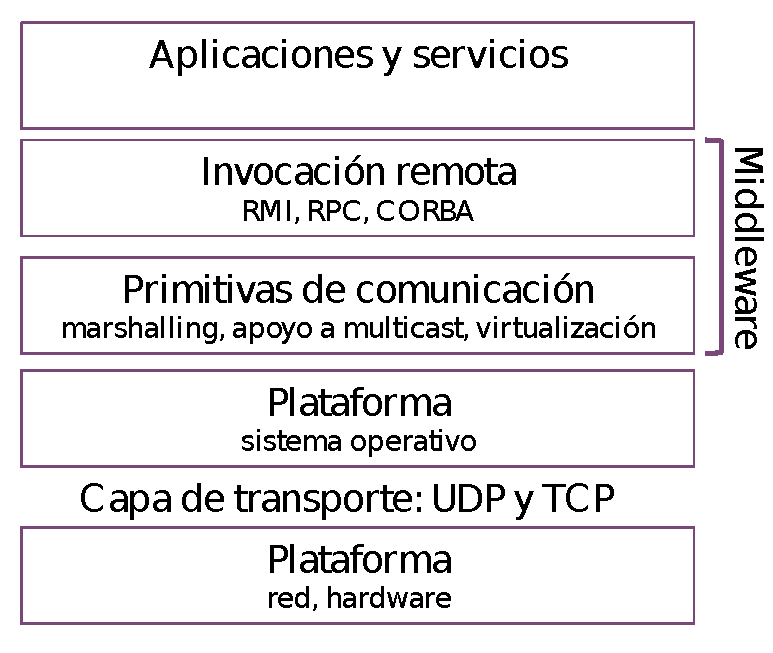
\includegraphics[width=0.4\textwidth]{Chapter2/Figures/middleware-rodrigo}
\caption{Ejemplo de una arquitectura que utiliza varias capas \textit{middleware}.}
\label{fig:middleware-rodrigo}
\end{figure}

\subsubsection{Utilización en el sistema final}

%TODO
Los diferentes \textit{bindings} de MarcoPolo (ver \ref{marcopolo:bindings}) pueden ser considerados middleware, pues abstraen los diferentes procesos de comunicación que ocurren al utilizar el sistema, proporcionando una interfaz independiente del lenguaje de programación y el sistema operativo. La serialización de las peticiones puede ser considerada \textit{middleware}.

Si \textbf{nsswitch} (ver \ref{nsswitch}) es considerado un sistema que abstrae los diferentes mecanismos de autenticación y resolución de nombres de la implementación de los mismos puede ser considerado un \textit{middleware}. \textbf{Nsswitch} se utiliza como método de abstracción de los diferentes proveedores de información de usuarios (archivos del sistema y \textbf{LDAP}) en el sistema final.

\subsection{Modelos arquitectónicos}

Existe un gran rango de diferentes modelos de construcción de sistemas distribuidos en función de las necesidades a cubrir por el sistema.

%TODO: Tanenbaum 2.1

\subsubsection{Clúster}

En general se conoce como clúster al conjunto de nodos homogéneos y dispuestos físicamente en la misma localización, conectados entre sí mediante mecanismos fiables como redes de área local y que cuentan con el mismo conjunto de herramientas (en particular el sistema operativo). Generalmente estos sistemas se componen de nodos de bajo coste, como equipos \textbf{COTS} y son utilizados para la realización de una única tarea con un coste computacional alto en paralelo.

\write18{wget -O Chapters/Chapter2/Figures/Beowulf.png -nc  http://upload.wikimedia.org/wikipedia/commons/4/40/Beowulf.png?download}

\begin{figure}[H]
  \centering
  \includegraphics[width=0.7\textwidth]{Chapter2/Figures/Beowulf.png}
  \caption[Beowulf]{Esquema de un clúster Beowulf. Este tipo de clústeres permiten obtener una gran capacidad de cómputo paralelo con equipos de bajo coste, y generalmente se comportan como una única unidad.}
\label{fig:beowulf}
\end{figure}

\subsubsection{\textit{Grid}}

Una ``rejilla'' (grid) es un sistema distribuido en el que los nodos del sistema no son homogéneos. Los mecanismos de transparencia descritos anteriormente son clave para el correcto funcionamiento del sistema y las interconexión entre los diferentes elementos.

\subsubsection{Sistemas de información distribuida}
%TODO
\citationneeded

\subsubsection{Sistemas descentralizados}

Uno de los principales problemas de las arquitecturas propuestas es la dependencia de un nodo que actúe de coordinador del resto. Dicha dependencia dificulta o incluso impide el funcionamiento del conjunto de nodos en caso de que el coordinador no cumpla adecuadamente su cometido (debido a fallos en el mismo, dificultades en la comunicación, etcétera). Las arquitecturas \textit{peer-to-peer} (de igual a igual) proponen una solución a dicho problema. Este tipo de enfoques flexibilizan la escalabilidad y tolerancia a fallos del sistema, si bien incorpora una serie de desafíos adicionales. La falta de coordinador implica que los diferentes nodos deben conocerse unos a otros previamente, o de algún modo descubrir la presencia del resto antes de poder cooperar. La centralización de dicho proceso es una de las soluciones propuestas para facilitar la construcción de la red de \textit{peers}\citationneeded.

Una de las ventajas de este tipo de sistemas es la facilidad para el establecimiento de redundancias, tanto de datos como de servicios, así como la alta tolerancia a fallos (el fallo de un nodo no impide que el resto pueda continuar su cometido a menos que cuente con una serie de recursos exclusivos).


\subsubsection{Utilización en el sistema final}

El sistema final es de tipo descentralizado, únicamente existiendo un coordinador en aquellos servicios en los que sea necesaria la presencia de uno (todos los nodos son capaces de actuar en ambos roles, y la elección del coordinador se realiza de forma distribuida, por lo que el fallo de un coordinador no supone un fallo total del sistema, y la recuperación es relativamente sencilla). Se utiliza el protocolo \textbf{MarcoPolo} (ver \ref{marcopolo}) para el descubrimiento de nodos y servicios, por lo que la configuración necesaria en el sistema es mínima.

\subsection{Seguridad}

Las medidas de seguridad a tomar dependen de las propiedades y objetivos propios del sistema: en general sistemas utilizados dentro de una organización y una infraestructura sin interacción con entornos no controlados suelen contar con un número menor de medidas de seguridad que aquellos utilizados en entornos ``hostiles'' (generalmente abiertos al público), y la seguridad depende de la confianza depositada en la administración del sistema. Sin embargo, un sistema de este tipo es vulnerable a ataques internos por parte de usuarios o intrusiones en la infraestructura.

Un sistema integrado en un entorno hostil debe además vigilar cualquier tipo de potencial ataque malicioso y controlar el acceso al sistema de forma más minuciosa.

\subsection{Protocolo}

Un protocolo consiste en un conjunto de formatos y reglas bien definidas y conocidas que son utilizadas para posibilitar la comunicación entre un conjunto de entidades. Un protocolo consta de dos especificaciones: la secuencia de mensajes que deben ser intercambiados en cada una de las diferentes acciones y la especificación del contenido y formato de dichos mensajes.

Si un protocolo es definido de forma correcta posibilitará la comunicación entre entidades sin importar la implementación del mismo, ofreciendo un alto grado de transferencia. De esta forma es posible, por ejemplo, ofrecer un servicio web que procese una serie de datos numéricos sin importar el tipo de \textit{endianness} del cliente o el servidor o el lenguaje de programación en el que el servicio se implementa. Únicamente es necesario conocer el tipo de dato que requiere el servicio y el valor esperado de retorno, así como los mensajes a intercambiar.

\subsubsection{Utilización en el sistema final}
%TODO
En el sistema se utilizan gran cantidad de protocolos conocidos (tales como HTTP, JSON, Websockets\dots) y se ha definido el protocolo de descubrimiento de servicios \textbf{MarcoPolo}.

\subsection{Integridad}

\subsection{Comunicación}

\subsection{Distribución}

Uno de los modelos típicos en el desarrollo de sistemas distribuidos es el ``divide y vencerás'': la división de un problema en múltiples tareas y la distribución de las mismas entre los diferentes componentes del sistema, reagrupando los resultados posteriormente. Dicho paradigma no se aplica únicamente a tarea a realizar, sino también al conjunto de datos sobre el que realizarla, paralelizando una misma operación en diferentes nodos sobre fragmentos del conjunto de datos sobre el que operar, recopilando los datos devueltos y conformando la respuesta final.

\write18{wget -P Chapters/Chapter2/Figures/ -nc http://upload.wikimedia.org/wikipedia/commons/6/6d/Mapreduce.png}

\begin{figure}[H]
  \centering
  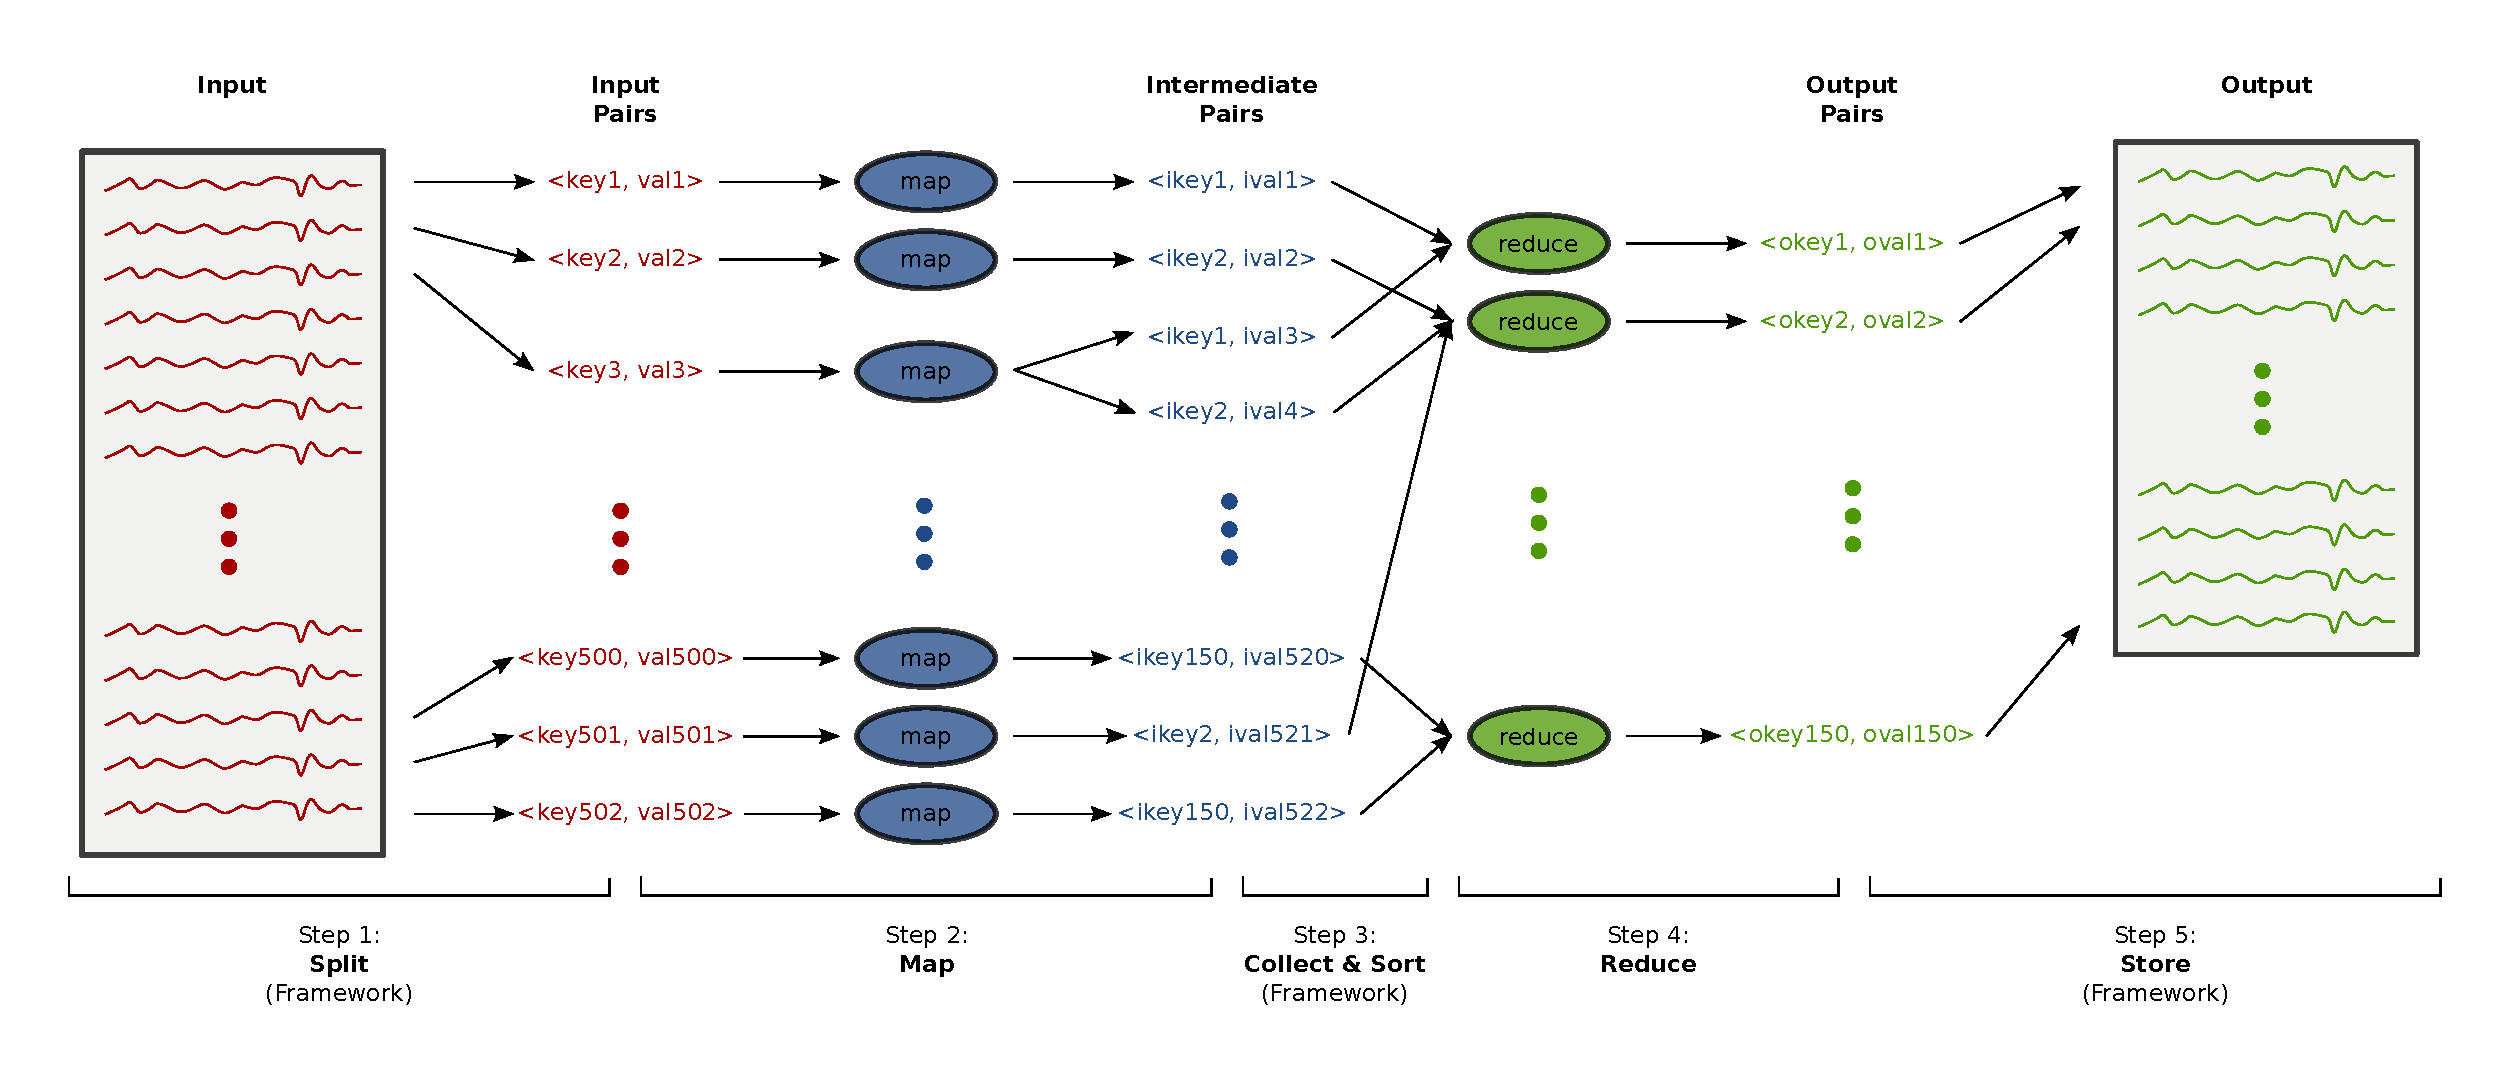
\includegraphics[width=0.85\textwidth]{Chapter2/Figures/map-reduce}
  \caption[MapReduce]{\textbf{MapReduce} se basa en el principio de la distribución de los datos sobre diferentes nodos (\textit{Map}) y la recopilación de los datos procesados (\textit{Reduce})}
  \label{fig:mapreduce}
\end{figure}

\subsection{Autoadministración}
\label{teoria:autoadministracion}

Un sistema distribuido debe proporcionar mecanismos que resuelvan de forma transparente todos los problemas asociados con la gestión de los mecanismos de interconexión entre los diferentes integrantes. Dichos mecanismos están diseñados para ser adaptativos y si bien el diseño suele ser genérico, es habitual encontrar soluciones \textit{ad-hoc}.

\subsubsection{Utilización en el sistema final}
%TODO: Polousers

\section{Paradigmas de programación}

\subsection{Programación orientada a eventos}
\label{teoria:eventdriven}

La programación orientada a eventos (\textit{event-driven programming}) constituye un patrón de programación en el cual el flujo del programa no se define íntegramente de forma secuencial, sino por las diversas interacciones (eventos) que el \textit{software} recibe durante su ejecución. Dichos eventos, generalmente impredecibles, son causados por cualquier otra aplicación o entidad externa, y su naturaleza es muy variada. Interacciones de ratón o teclado, conexiones de red o estímulos de sensores son claros ejemplos, pero también son eventos notificaciones de finalización de un trabajo o llamadas periódicas.

La programación orientada a eventos es un patrón exitoso en varios tipos de aplicaciones, en particular aquellas con interfaz gráfica de usuario, donde la interacción es completamente imprevisible o aplicaciones de un único hilo (\textit{single-threaded applications}), que utilizan los eventos para establecer mecanismos de coordinación. 

Si bien existen una gran cantidad de herramientas para el desarrollo de \textit{software} siguiendo este patrón, el funcionamiento de todas ellas se reduce a un conjunto de manejadores y disparadores de eventos. También reciben nombres similares, como señales y ranuras.

\subsubsection{Suscriptor de eventos}

Un suscriptor de eventos permite vincular un evento a un manejador (\textit{handler}), que determina la acción a realizar al recibir un evento. En una gran cantidad de \textit{frameworks} se definen como funciones. Por ejemplo:

\begin{figure}[H]
\centering
  \begin{lstlisting}
  function manejadorMouseMove(evento){
    console.log(evento.pageX);
  }
  document.onmousemove=manejadorMouseMove
  \end{lstlisting}
\caption[Evento y manejador]{El evento ``onmousemove'', que se dispara en el momento en el que el ratón se desplaza, es vinculado a la función \texttt{manejadorMouseMove} en una página web.}
\end{figure}


Ejemplos de herramientas que utilicen este paradigma son \textbf{Node.js}, \textbf{Tornado web}, \textbf{Twisted} o la gran mayoría de los \textit{frameworks} para creación de interfaces gráficas, como \textbf{Cocoa}, \textbf{Windows Presentation Framework} o \textbf{Qt}, entre otros.

En el proyecto se utiliza este patrón para la creación de la mayoría de las herramientas, en particular en combinación con el modelo de aplicaciones de un único hilo (ver \ref{teoria:singlethread}).

\subsection{Paralelización, hilos y procesos}

Uno de los mecanismos para conseguir paralelizar tareas es su distribución en procesos independientes. Cada proceso cuenta con un espacio de memoria y asignación de recursos por parte del sistema operativo (CPU, descriptores de fichero abiertos\dots) completamente independiente. Sin embargo, dicha independencia implica la reserva de un segmento de memoria y el almacenamiento de los valores de ejecución (contador de programa, valores de registros, puntero de pila, etcétera) cuando la CPU debe realizar un cambio de contexto para permitir la ejecución de otro proceso. Dicha alternancia y la reserva de estos recursos implican un coste computacional en ocasiones alto, en particular cuando el número de cambios de contexto es elevado. Como solución se plantea el uso de hilos (\textit{threads}), ejecuciones de fragmentos de código independientes del resto de hilos pero con un nivel de transparencia menor si el mantenimiento de la misma afecta al rendimiento del conjunto de hilos.

\label{teoria:singlethread}
Un tercer enfoque es desarrollo de aplicaciones dirigidas por eventos (\textit{event-driven}) en un único hilo (\textit{single-threaded application}). Para conseguir paralelizar las diferentes tareas se deben ejecutar de forma no bloqueante, cediendo la CPU a otra tarea en caso de que se deba esperar a que otra sea realizada (generalmente, operaciones de entrada-salida, que presentan un gran tiempo de espera sin consumo de CPU, como la descarga de información en red o el acceso al almacenamiento secundario).

%TODO: Node I/O example

Mediante rellamadas (\textit{callbacks}) una tarea que termina una operación de este tipo indica al hilo gestor que requiere de nuevo tiempo de computación, y este añadirá la tarea de nuevo a la cola de acceso a la CPU.

\begin{figure}[H]
  \centering
  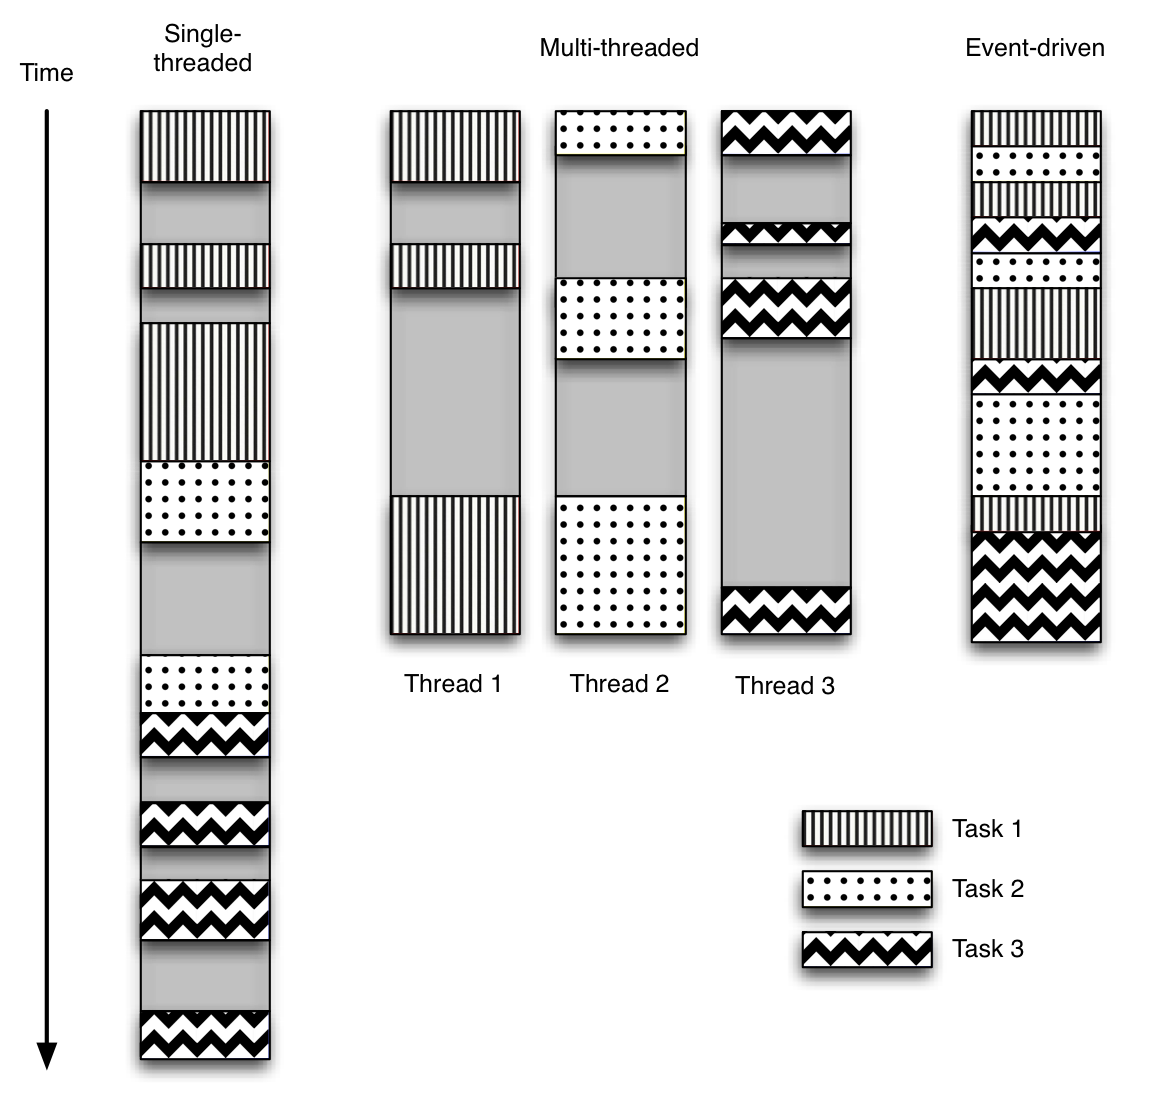
\includegraphics[width=0.7\textwidth]{Chapter2/Figures/threadcomparison}
  \caption[Modelos de paralelización]{Comparación de los diferentes modelos de paralelización\citationneeded[Twisted book]}
  \label{fig:threadcomparison}
\end{figure}

\subsubsection{Patrón Reactor}

El patrón de diseño reactor\cite{Coplien95reactor} consiste en un sistema de gestión de peticiones de servicio distribuidas de forma concurrente en un esquema cliente-servidor. En el servidor existe un manejador de eventos que distribuye (demultiplexa) los diferentes eventos a manejadores de los mismos, distribuyendo el tiempo de proceso entre ellos de forma síncrona mediante un bucle ejecutado de forma continua.

\begin{figure}[H]
  \centering
  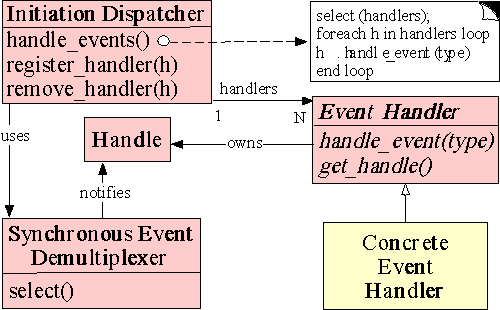
\includegraphics[width=0.6\textwidth]{Chapter2/Figures/reactoruml}
  \caption[Diagrama UML del patrón reactor]{Diagrama UML del patrón reactor\label{Coplien95reactor}.}
  \label{fig:reactoruml}
\end{figure}




\section{Sincronización}

\subsection{Mecanismos de coordinación}

En determinadas ocasiones es necesaria la presencia de un coordinador que lleve a cabo una serie de tareas de gobierno. La elección de dicho coordinador puede atender a una serie de criterios muy variados y los mecanismos de designación siguen varios enfoques:

\subsubsection{Coordinación central}

Un nodo, o instancia de un programa es designado como coordinador, cuya autoridad es obedecida por el resto de integrantes del sistema. Es un enfoque sencillo de implementar que sin embargo crea un punto de fallo en el sistema, pues la caída del coordinador central impedirá la realización de cualquier tarea en la que sea necesaria su intervención hasta que vuelva a estar activo.

El coordinador puede designarse mediante diferentes mecanismos. En algoritmos como OSPF\cite{rfc2328} la política de elección del \textit{router} designado es aquel que cuente con el mayor valor de prioridad.
%TODO: Completar
\subsubsection{Coordinación distribuida}

Con objeto de solventar los problemas que la coordinación centralizada conlleva se proponen algoritmos que permiten designar un coordinador y reemplazarlo en caso de fallo del mismo.

\paragraph{Algoritmo del abusón}

El algoritmo del abusón (descrito en \cite{Coulouris:2011:DSC:2029110:Ch15}) posibilita la elección de un coordinador en función del cumplimiento de un criterio cuantitativo dado, siendo elegido coordinador aquel que mejor satisfaga dicho criterio. La secuencia de pasos es la siguiente:

Sea un proceso, \textit{P} que detecta la ausencia de un coordinador (en caso de que ya se haya ejecutado el algoritmo, se detecta la ausencia del anterior coordinador) y \textit{X} un valor numérico que determina el criterio para la elección del coordinador (el proceso con el valor más alto te \textit{X} será el coordinador).
\begin{enumerate}
\item \textit{P} envía un mensaje de elección a todos los procesos con \textit{X} más alto que \textit{X\textsuperscript{P}}.
\item Si ningún proceso responde en un tiempo dado, \textit{P} envía un mensaje indicando que es el coordinador.
\item En caso de que algún proceso responda al mensaje, el proceso se repetirá con el conjunto de nodos con \textit{X} mayor que \textit{X\textsuperscript{P}}.
\end{enumerate}

\begin{figure}[H]
  \centering
  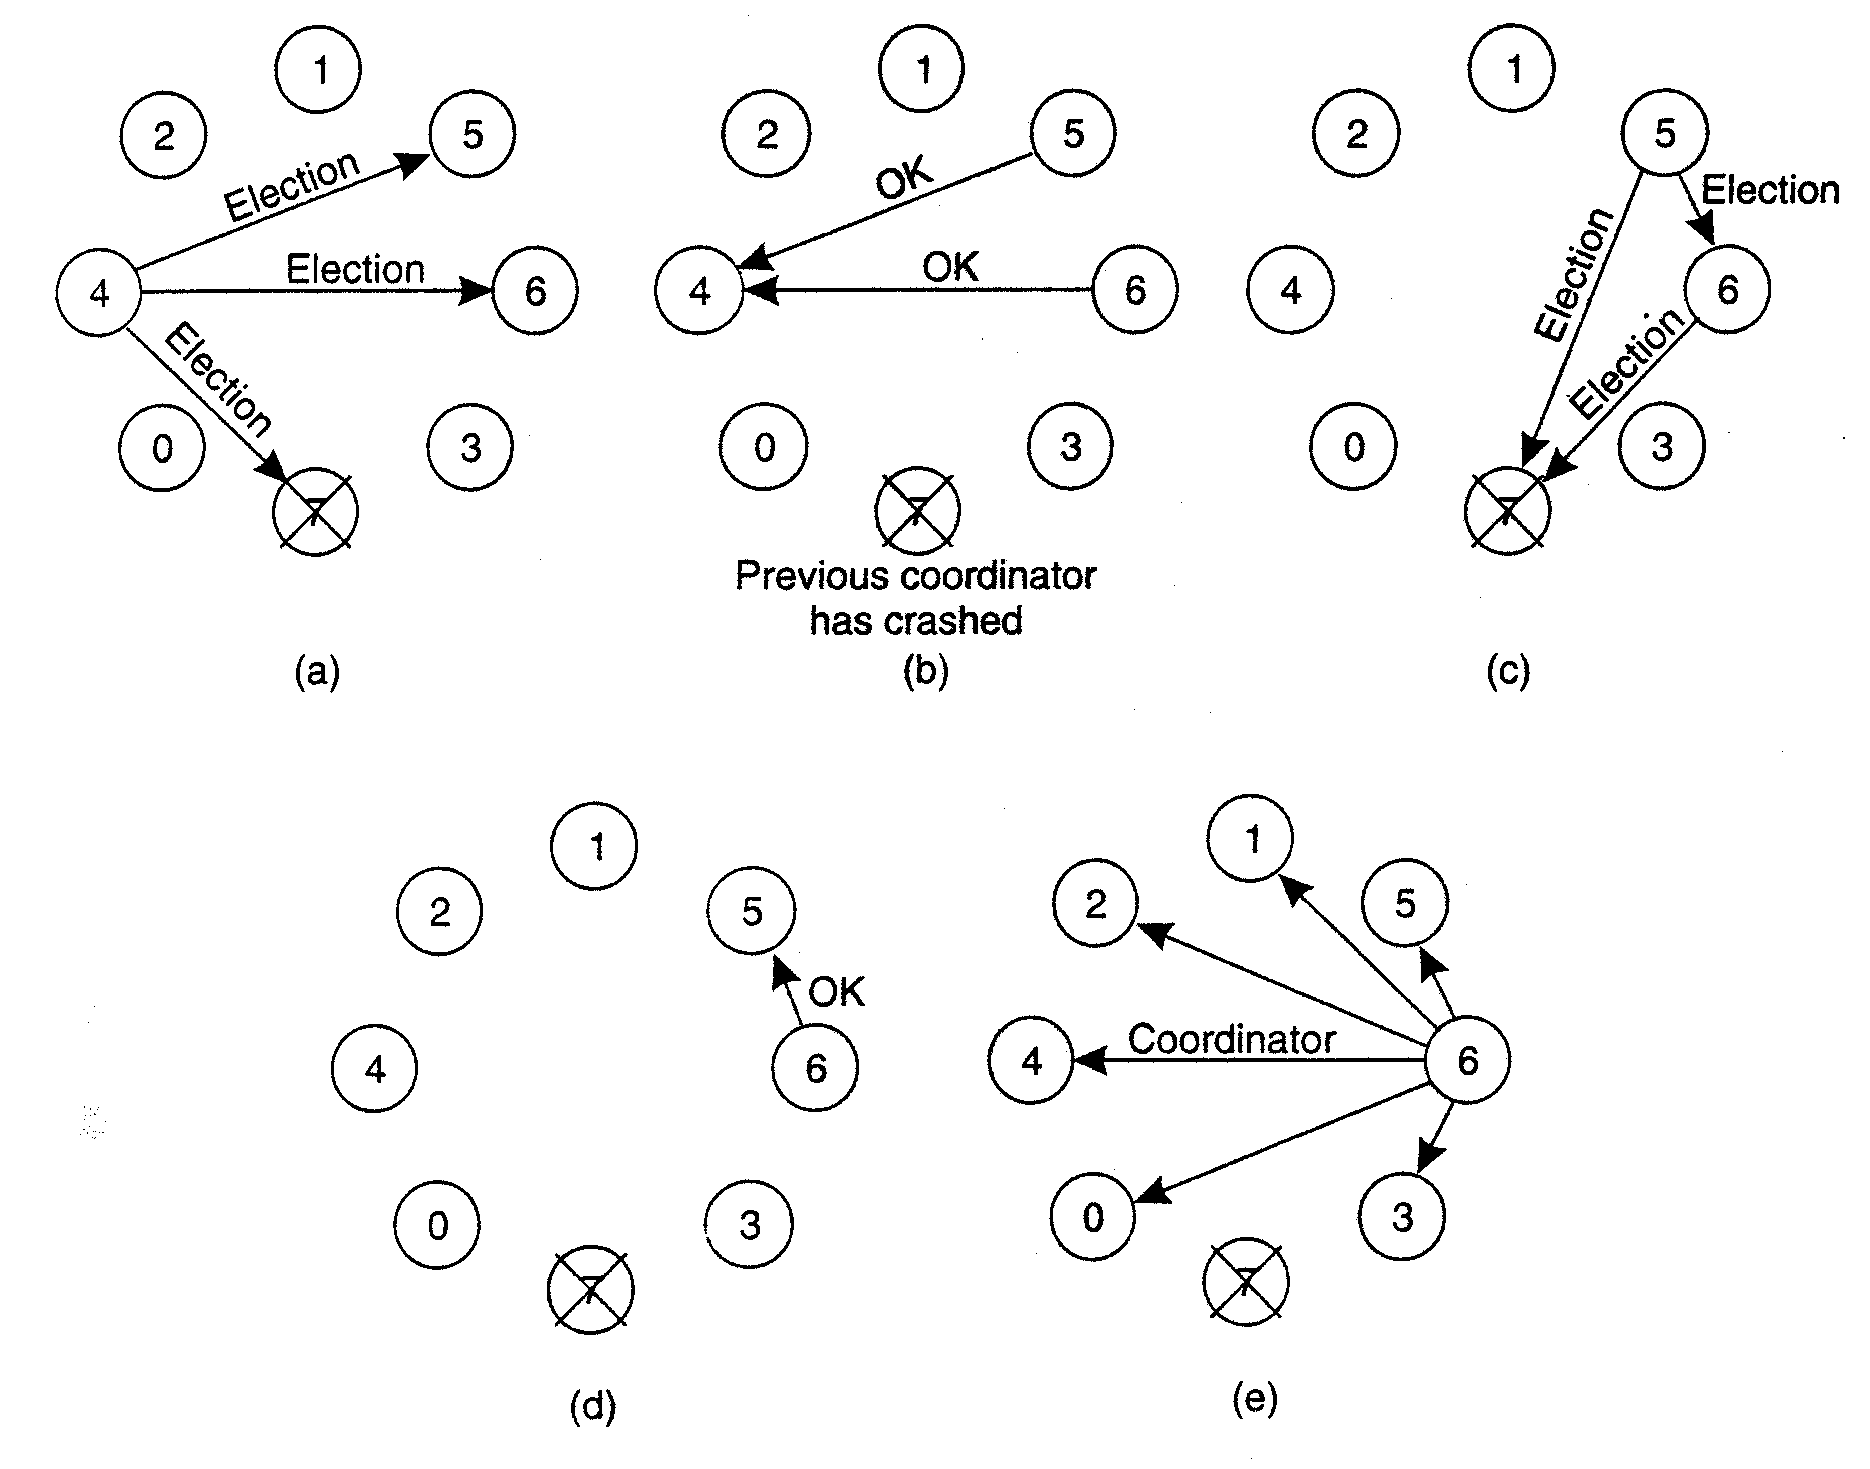
\includegraphics[width=0.8\textwidth]{Chapter2/Figures/bully}
  \caption{Secuencia de elección de un coordinador}
  \label{fig:tanenbaum:bully}
\end{figure}

\paragraph{Algoritmo en anillo}

El algoritmo funciona bajo la premisa de que todos los procesos cuentan con un orden preestablecido, conociendo a su antecesor y sucesor en la cadena\cite{Tanenbaum:2006:DSP:1202502:Ch6}. El funcionamiento del algoritmo es el siguiente:

\begin{enumerate}
  \item Cuando un proceso \textit{P} detecta la caída de un coordinador, envía un mensaje de elección al proceso sucesor, o en su defecto, al proceso sucesor más próximo, en caso de que se encuentre inactivo, hasta que encuentre un proceso activo.
  \item Cuando un proceso recibe el mensaje, añade al mismo su número de proceso.
  \item Una vez que el mensaje llega al creador del mismo, este construye un mensaje con el identificador del proceso que ha sido elegido como coordinador (el proceso con el identificador más alto, o aquel que satisfaga otro criterio similar) y lo envía al siguiente proceso de manera similar al mensaje inicial, si bien el contenido del mensaje no es alterado en este caso.
  \item Una vez que el mensaje ha circulado por todos los procesos, retorna a su creador y en este momento el trabajo se reanuda.
\end{enumerate}

\begin{figure}[H]
  \centering
  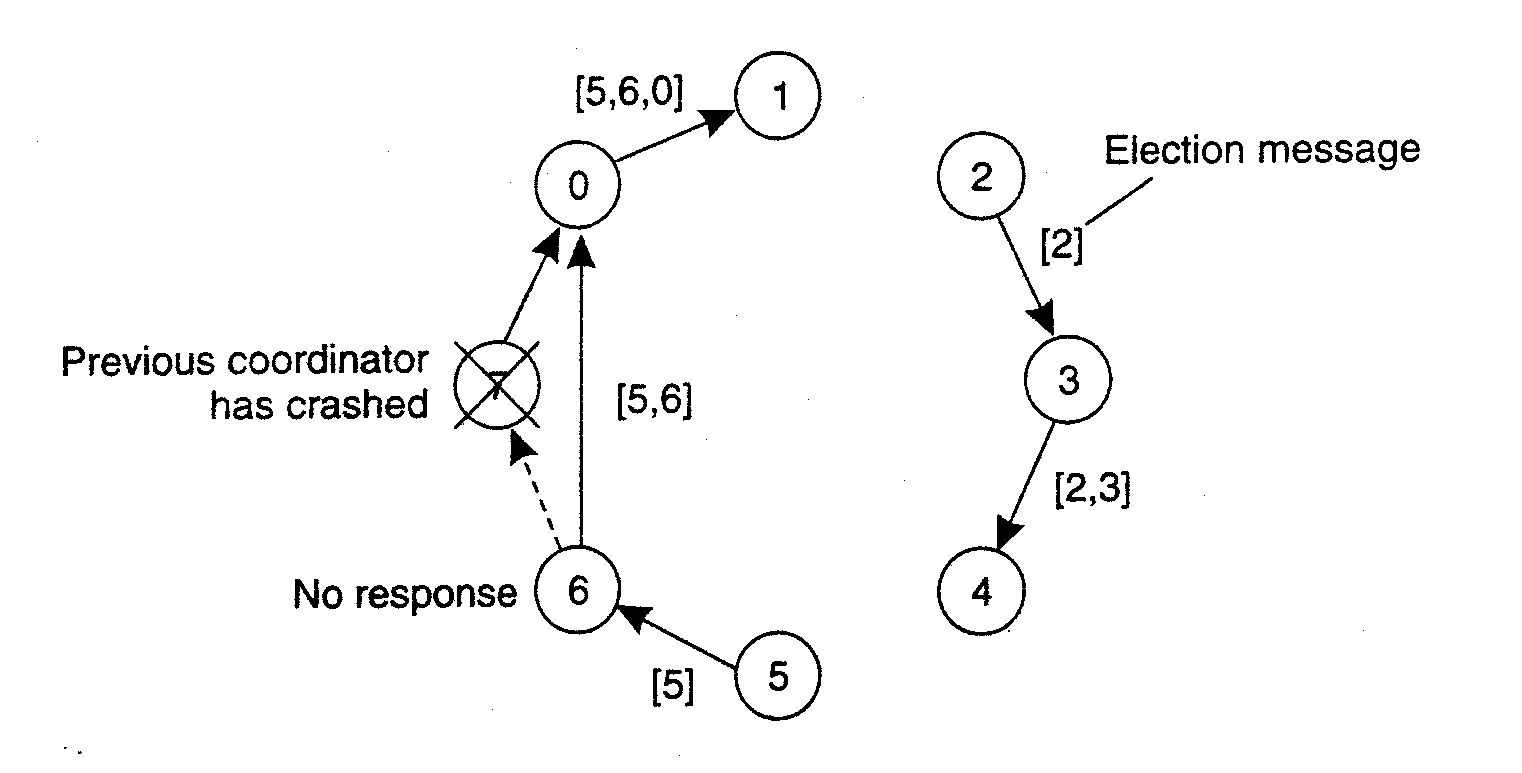
\includegraphics[width=0.8\textwidth]{Chapter2/Figures/ringalgorithm}
  \caption{Funcionamiento del algoritmo en anillo}
  \label{fig:tanenbaum:ringalgoritm}
\end{figure} 

%DOCKER

\section{Protocolos criptográficos}

\subsection{Criptografía asimétrica}

La criptografía asimétrica, o criptografía de clave pública se basa en algoritmos que requieren un par de claves en cada entidad, siendo una de ellas conocida únicamente por dicha entidad (clave privada) y la otra públicamente disponible. Dichos algoritmos se basan en problemas sin solución en un tiempo aceptable, como por ejemplo la factorización de enteros.

Ambas claves consisten en un valor numérico y están relacionadas matemáticamente entre sí. La clave pública es utilizada para realizar operaciones de cifrado de datos o verificación de una firma digital, mientras que la clave privada es utilizada para los procesos complementarios.

\subsection{Infraestructura de clave pública}

Una infraestructura de clave pública está formada por el conjunto de \textit{hardware}, \textit{software}, políticas y procedimientos necesario para la creación y gestión de certificados digitales, documentos electrónicos utilizados para probar la identidad de una determinada entidad. Dichas infraestructuras se componen de una autoridad (\textbf{CA}, \textit{Certificate Authority}) que garantiza la identidad del solicitante de un certificado, y por tanto, es el responsable de verificar dicha identidad en el momento de creación del mismo. El resto de entidades confiarán en dicha \textbf{CA}. Estos certificados se componen de un par de claves pública y privada\citationneeded.

\subsubsection{X.509}

El estándar X.509\label{rfc4158} define una realización de una infraestructura de clave pública en la cual los certificados están vinculados a un nombre, sea este un nombre distinguido (siguiendo la estructura del protocolo LDAP, ver \ref{teoria:ldap}) o un nombre alternativo, como una dirección de correo electrónico o un nombre \textbf{DNS}. Según el estándar se define una cadena de validación que culmina en los denominados certificados raíz, a partir de los cuales son creados el resto de autoridades de certificación y finalmente, los certificados dados a los diferentes componentes que los utilizan.

La estructura de un certificado es la siguiente\label{rfc5280}:

\begin{itemize}
  \item Certificado.
    \subitem Versión.
    \subitem Número de serie.
    \subitem Tipo de algoritmo.
    \subitem Distribuidor.
    \subitem Validez.
      \subsubitem No válido hasta.
      \subsubitem No válido después de.
    \subitem Información de clave pública: Algoritmo y clave.
    \subitem Identificador único del distribuidor (opcional).
    \subitem Identificador único del solicitante (opcional).
    \subitem Extensiones (opcional).
  \item Algoritmo de firma del certificado.
  \item Firma del certificado.
\end{itemize}

\subsection{TLS/SSL}
El protocolo \textit{Transport Layer Security}\cite{rfc5246} y su predecesor, \textit{Sockets Security Layer} permiten establecer conexiones seguras sobre un canal inseguro (proclive a ataques pasivos como el uso de \textit{sniffing}\citationneeded o activos, como técnicas de \textit{spoofing} o \textit{man-in-the-middle}\citationneeded) mediante el uso de una infraestructura de clave pública. Este protocolo se integra en los niveles de sesión y presentación del modelo OSI, y por lo tanto utilizan los mismos protocolos de transporte y red que una conexión tradicional, por lo que es sencillo construir aplicaciones sobre canales seguros utilizando las mismas técnicas que las usadas en este tipo de comunicaciones, o incluso reutilizar código. El protocolo funciona según la siguiente secuencia:

\begin{enumerate}
\item El proceso con el rol de cliente comienza el proceso conocido como ``apretón de manos'' (\textit{handshake}, solicitando una conexión segura junto con las diferentes funciones de cifrado admitidas).
\item El servidor elige una de las funciones propuestas y notifica la decisión al cliente.
\item El servidor envía su identificación en forma de certificado digital, que incluye campos como su \textit{common name}, la autoridad de certificación y la clave pública.
\item El cliente valida la autoridad de certificación según la cadena de validación presente en el mismo, o en caso necesario, contactando a esta.
\item El cliente cifra un número aleatorio con la clave pública del servidor y se lo envía.
\item Mediante este número se genera la clave simétrica secreta (``secreto maestro'') y negocian una clave de sesión para realizar los procesos de cifrado.
\item Comienza la transmisión de información.
\end{enumerate}

En caso de que alguno de los pasos sea infructuoso, la conexión terminará. 

\subsection{HTTPS}

El protocolo HTTPS\cite{rfc2818} utiliza TLS para cifrar las conexiones realizadas mediante el protocolo HTTP. La combinación de ambos protocolos se realiza superponiendo TLS al protocolo HTTP, por lo que las cabeceras y datos transmitidos no son alterados, siendo por tanto compatibles entre sí. Este protocolo (o combinación de protocolos, al consistir en la simple combinación de varios) es utilizado en recursos web para garantizar la identidad del servidor que envía los datos y establecer un canal seguro sobre una red no segura.

\subsection{Autenticación mutua}
\label{teoria:autenticacionmutua}
El uso más común de los protocolos previamente definidos es verificar la identidad del servidor al que se está conectando un cliente. Sin embargo, en ocasiones es necesario que el servidor confíe en el cliente, como en situaciones donde el cliente no dispone de otro mecanismo de autenticación, como puede ser un par usuario-contraseña. El \textit{handshake} es similar al utilizado tradicionalmente, únicamente se añade el paso de validación del certificado que el cliente debe enviar al servidor.

En el sistema este proceso de autenticación se utiliza en aquellas aplicaciones sin interfaz de usuario o que realizan operaciones que puedan comprometer la integridad del sistema de forma significativa (por ejemplo, solicitar la realización de operaciones con privilegios de administrador en \textbf{pam\_mkpolohomedir} o la descarga de un sistema operativo que contiene todas las claves privadas, que deben ser confidenciales).

\section{Autenticación}
\subsection{PAM}

El \textit{Linux Pluggable Authentication Module}\cite{opengroup:rfc86.0} es un componente integrable en el mecanismo de autenticación del sistema operativo para combinar diferentes mecanismos de identificación que puedan ser aprovechados por aplicaciones de alto nivel, abstrayendo las características del sistema de autenticación presente en la máquina, proporcionando una interfaz única. \textbf{PAM} se apoya en diferentes fuentes de datos configurables, tales como los ficheros \texttt{/etc/passwd} y \textbf{/etc/shadow}, directorios \textbf{LDAP} (ver \ref{teoria:ldap}), autenticación mediante clave pública, (ver \ref{teoria:ldap}).

\begin{figure}[H]
\centering
  \immediate\write18{if ! [ -f Chapters/Chapter2/Figures/pamstructure.png ];then wget -O Chapters/Chapter2/Figures/pamstructure.gif -nc http://pubs.opengroup.org/onlinepubs/8329799/sso0401.gif; convert Chapters/Chapter2/Figures/pamstructure.gif Chapters/Chapter2/Figures/pamstructure.png;rm Chapters/Chapter2/Figures/pamstructure.gif;fi}
  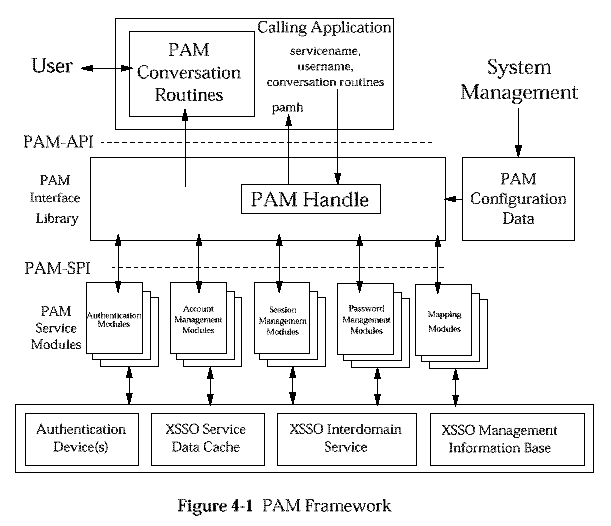
\includegraphics[width=0.6\textwidth]{Chapter2/Figures/pamstructure.png}
  \caption[Esquema de la arquitectura de PAM]{Esquema de la arquitectura de PAM (fuente \cite{opengroup:rfc86.0})}
\end{figure}

PAM está diseñado para definir su comportamiento mediante el uso de módulos, pequeñas piezas de código que definen las acciones a llevar a cabo dadas un conjunto de circunstancias, como el cambio de una contraseña, la modificación de un parámetro en la información del usuario o el acceso al sistema de un usuario. Mediante los parámetros de configuración de \textbf{PAM} se definen aquellas circunstancias que requieren del uso del módulo definido.

\begin{figure}[H]
\centering
\begin{lstlisting}
service module_type control_flag module_path         options
------- ----------- ------------ -----------         -------
login   auth        required     pam_unix_auth.so    nowarn
login   session     required     pam_unix_session.so
login   account     required     pam_unix_account.so
ftp     auth        required     pam_skey_auth.so    debug
ftp     session     required     pam_unix_session.so
telnet  session     required     pam_unix_session.so
login   password    required     pam_unix_passwd.so
passwd  password    required     pam_unix_passwd.so
OTHER   auth        required     pam_unix_auth.so
OTHER   session     required     pam_unix_session.so
OTHER   account     required     pam_unix_account.so
\end{lstlisting}

\caption[Fichero de configuración de PAM]{Un fichero de configuración de PAM con diferentes módulos definidos para el acceso al sistema mediante un terminal (\textit{login}), FTP, Kerberos o telnet, así como acciones a realizar cuando una entrada del fichero \texttt{/etc/passwd} es modificada (\textit{passwd})}.
\end{figure}

\subsection{LDAP}
\label{teoria:ldap}

El protocolo \textit{Lightweight Directory Access Protocol} posibilita el acceso a directorios de información en un entorno distribuido siguiendo un esquema cliente-servidor.

%TODO: http://es.wikipedia.org/wiki/Protocolo_Ligero_de_Acceso_a_Directorios. Incluir los campos necesarios para explicar X.509

\subsubsection{Utilización en el sistema final}

La gestión de usuarios está delegada al módulo PAM, utilizando los mecanismos de autenticación que provee en las diferentes aplicaciones del sistema, como en \textbf{Deployer}.

Con el objetivo de garantizar diversas propiedades de transparencia del sistema, se ha creado un módulo de PAM que se integra con \textbf{MarcoPolo} para la realización de tareas de gestión en el conjunto de nodos del sistema (ver \ref{pam_mkpolohomedir}).

\section{Comunicación}

La comunicación entre procesos dentro de un sistema distribuido constituye un aspecto clave en el diseño del mismo, y existen una gran cantidad de modelos para posibilitarlo.

\subsection{Multicasting}

Si bien las comunicaciones punto a punto consituyen un mecanismo efectivo para la comunicación entre diferentes nodos, presentan una serie de ineficiencias a la hora de distribuir el mismo contenido entre un número significativo de nodos, al tener que enviar un mensaje diferente a cada uno de los destinatarios. Utilizar difusión (\textit{broadcast}) para este tipo de aplicaciones supone una alternativa efectiva, si bien obliga a las entidades no interesadas en el mensaje a procesar el mismo en ocasiones hasta el nivel de red de la pila OSI \citationneeded.

Como alternativa surge la comunicación \textit{multicast} sobre el protocolo IP. Este tipo de mensajes son enviados a una dirección en un rango reservado (en IPv4, 224.0.0.0-239.255.255.255, las direcciones con el valor 1110 en el primer octeto, conocidas como Clase D\cite{rfc791}), conocido como \textit{grupo}. Los nodos interesados en los mensajes publicados en dicho grupo pueden suscribirse al grupo multicast y cancelar su membresía en cualquier momento dado. Todos los mensajes son de tipo UDP, si bien existen extensiones al protocolo TCP para posibilitar su uso en aplicaciones multicast, si bien de forma experimental\cite{1019386, mysore2001ftp, Barcellos01efficienttcp-like, Visoottiviseth01m/tcp:the, talpadereliablemulticast} o soluciones que permiten realizar multicast fiable (con diferentes grados de fiabilidad) sobre UDP\cite{rfc2887}.

\subsection{Serialización}
\label{seralization}
Con el objetivo de posibilitar la intercomunicación entre entidades es necesario determinar mecanismos para la representación de estructuras de datos complejas de forma homogénea, definiendo una serie de reglas para la representación de datos sin importar la plataforma de cada una de las diferentes entidades partícipes.

Existen una serie de formatos definidos que posibilitan este tipo de interconexión. Uno de ellos es \textbf{JSON} (\textit{JavaScript Object Notation})\cite{rfc7159}. \textbf{JSON} define estructuras de datos complejas, tales como objetos, listas o diccionarios clave-valor, mediante un subconjunto de la sintaxis de \textbf{JavaScript} que permite representar cualquier tipo de dato de forma legible por personas y fácilmente comprensible por máquinas. Existen implementaciones de procesadores de JSON en la mayoría de lenguajes de programación, lo cual permite el intercambio de información entre diferentes programas de forma sencilla.

\subsubsection{Utilización en el sistema final}

Toda comunicación entre dos entidades se realiza gracias a cadenas con formato \textbf{JSON} (salvo casos concretos, como los programas ejecutados sobre MPI, donde el entorno proporciona un mecanismo claramente más efectivo de comunicación) utilizando bibliotecas de terceros para el procesamiento de las mismas.

\subsection{WebSockets}
%TODO

\section{Modelos de desarrollo}
\subsection{Test-Driven Development}
\label{tdd}

El desarrollo dirigido por pruebas es una estrategia de desarrollo de software basada en el desarrollo de tests de partes concisas y fácilmente desacoplables del código de una aplicación que realizan una tarea muy concreta (conocidas como pruebas unitarias). Dichas pruebas se realizan generalmente con un control exhaustivo de las condiciones que pueden influir el desarrollo de la prueba. Mediante la modificación de dichas condiciones y el análisis de la respuesta frente a un conjunto de datos de entrada se puede analizar si el comportamiento de dicho fragmento de código es el adecuado.

Las pruebas consisten generalmente en una serie de aserciones sobre el resultado del fragmento de código ejecutado, o sobre un estado intermedio. Una batería de pruebas consistente debe cubrir el mayor número de resultados de salida posible, incluyendo valores que indiquen condiciones de error (verificando que dicho error deba ser devuelto para los parámetros de entrada y condiciones iniciales), excepciones y diferentes tipos de retorno válidos.

Un ciclo de desarrollo basado en pruebas consiste en dos fases: inicialmente la escritura de la batería de pruebas basadas en los diferentes requisitos del \textit{software} y ejecución de dicha batería, que deberá ser completamente infructuosa. Tras esta fase comienza la etapa de refactorización, consistente en la implementación de la funcionalidad que el fragmento de código de cada test debe realizar y la ejecución de la batería de pruebas durante las diferentes etapas de implementación. Cuando un test se ejecute satisfactoriamente se garantizará que el código cumple los requisitos de la prueba definidos en la fase inicial, y por tanto, con los requisitos del \textit{software}.

Esta práctica asiste al programador en el desarrollo de \textit{software} más fiable, pues todas las potenciales condiciones de fallo que se reflejan en la batería de pruebas son cubiertas durante la segunda fase del proceso (o en caso contrario el resultado test no será satisfactorio). Uno de los efectos secundarios del desarrollo dirigido por pruebas es la escritura de código de grano muy fino y muy desacoplado (al tener que desacoplar la funcionalidad para poder adaptarla a una prueba unitaria). El desarrollo dirigido por pruebas permite también controlar de forma sencilla las interdependencias entre diferentes módulos de código, pues basta con ejecutar la batería de tests tras una modificación de un componente del cual dependan otros para evaluar si dichos cambios afectan al comportamiento del resto de módulos.

Si bien la escritura de código siguiendo este modelo de desarrollo suele ser sencilla, en ocasiones se dan un conjunto de condiciones que dificultan significativamente el diseño de pruebas. Generalmente dichas condiciones están relacionadas con la modificación de entidades externas, como pueden ser bases de datos o recursos en red. Para dichos casos la mayoría de herramientas de creación de tests ofrecen funcionalidad para crear ``objetos simulados'' (\textit{mock}), objetos que simulan el comportamiento del elemento al que reemplazan pero evitando los efectos de los mismos (como la modificación de una base de datos o el envío o la recepción de un paquete en red). Dichos objetos permiten simular una serie de condiciones como valores de retorno o lanzamiento de excepciones, así como el análisis de los parámetros con los que es invocado (en caso de que el objeto \textit{mock} reemplace a una función o clase) o la inclusión de parámetros únicamente relevantes durante la fase de realización de pruebas.

\subsubsection{Utilización en el sistema final}

Varias de las las herramientas del Trabajo han sido desarrolladas siguiendo este proceso de desarrollo. No ha sido posible la aplicación en la construcción de la totalidad de las herramientas debido a la falta de conocimientos sobre este proceso de desarrollo hasta comenzar con el Trabajo. Sin embargo, se han escrito tests unitarios para casi la totalidad de las herramientas existentes anteriormente, utilizando el desarrollo dirigido por pruebas en sucesiones iteraciones dentro del ciclo de desarrollo de estas aplicaciones.



%TODO: PAM para cambiar el directorio HOME
\section{Otros}

\subsection{Virtualización}
\label{teoria:virtualizacion}

Virtualizar consiste en la abstracción de la plataforma física sobre la que un conjunto de \textit{software} es ejecutado. La virtualización de diferentes capas de un sistema facilita la compatibilidad entre componentes de características muy variadas, y posibilita la creación de diferentes unidades independientes sobre un único equipo físico, la abstracción de diferentes capas (hardware, sistema operativo, bibliotecas) de la implementación de la aplicación final.

\subsection{Código móvil}
\label{teoria:codigomovil}

Se conoce como código móvil al \textit{software} que se transfiere entre diferentes unidades (distribuido en una red, generalmente). Este tipo de aplicaciones ofrecen una serie de ventajas (principalmente la sencilla distribución del mismo, en ocasiones transparente al usuario final) muy atractivas a la hora de crear sistemas distribuidos.

La mayoría de este tipo de \textit{software} está creado sobre herramientas multiplataforma, garantizando la abstracción del sistema sobre el que se está ejecutando. Ejemplos de código móvil son los contenidos dinámicos de una web (creados mediante \textbf{applets} Java, código \textbf{JavaScript} o controles \textbf{ActiveX}), código embebido en documentos PDF o en general cualquier tipo de \textit{software} descargado de una red.

Sin embargo, este tipo de aplicaciones implican una serie de consideraciones adicionales de seguridad, en particular la verificación de la identidad del nodo que proporciona el paquete, la integridad del mismo durante la transferencia y \citationneeded y el comportamiento del código en ejecución.

\subsubsection{Compartimentación}

Extendiendo los conceptos del código móvil a un contexto más amplio, como el de un sistema operativo, surge la idea de la compartimentación, consistente en la creación de entornos (compartimentos) capaces de ser migrados incluso en tiempo de ejecución entre máquinas, evitando la interrupción de un trabajo en caso de que el nodo sobre el que se está ejecutando deba ser interrumpido, entre otros muchos beneficios.

\subsection{\textit{Cross-compiling}}

La compilación cruzada posibilita el desarrollo de \textit{software} en plataformas diferentes a la plataforma objetivo, aquella sobre la que el programa final deberá ejecutarse. El compilador genera código máquina para la arquitectura objetivo a partir de los archivos de código fuente, en lugar del proceso común de generación de código para la arquitectura sobre la que se ejecuta el software de desarrollo (proceso conocido como compilación nativa).

El uso de compiladores cruzados facilita el desarrollo para diferentes plataformas y en ocasiones es la única forma de crear aplicaciones para sistemas tales como dispositivos embebidos que no cuentan con herramientas de desarrollo. También es útil para facilitar la generación de código en entornos como granjas de servidores, generación de código para emuladores o realizar procesos de \textit{bootstrapping} (creación de las herramientas básicas de una nueva plataforma, como un sistema operativo o un enlazador).


\subsubsection{\textit{Toolchain}}

Una cadena de herramientas (\textit{toolchain}) se conforma del conjunto de utilidades necesarias para la construcción de un determinado producto. Generalmente estas utilidades son ejecutadas secuencialmente, utilizando la salida de una de ellas como la entrada de la siguiente. Este conjunto de herramientas comprende normalmente un compilador, un enlazador y un editor de texto, así como varias bibliotecas y un depurador, si bien puede contar con cualquier herramienta requerida para las necesidades propias del producto a crear.

\subsection{Utilización en el sistema final}
%\subsec
Con el objetivo de posibilitar la realización de trabajos de compilación distribuida utilizando un equipo basado en la arquitectura i686 %TODO: Revisar
se ha construido una cadena de herramientas que realiza procesos de compilación cruzada para la arquitectura ARMv7hf utilizando la herramienta \textit{crosstool-ng}\citationneeded, consiguiendo optimizar de forma significativa el tiempo de compilación.
%TODO (ver \ref{distcc:analysis})
%TODO: También existe una versión para la arquitectura ARMv6hf.
%TODO, además dicha herramienta se ha utilizado para la creación de una herramienta de desarrollo con Eclipse para Raspberry Pi.

\citationneeded{http://www.nongnu.org/avr-libc/user-manual/overview.html}
\citationneeded{http://elinux.org/Toolchains}
%TODO: http://en.wikipedia.org/wiki/Paravirtualization

